\documentclass[compress]{beamer}
\usepackage{ifthen,verbatim}

\newcommand{\isnote}{}
\xdefinecolor{lightyellow}{rgb}{1.,1.,0.25}
\xdefinecolor{darkblue}{rgb}{0.1,0.1,0.7}
\xdefinecolor{darkred}{rgb}{0.9,0.,0.}
\xdefinecolor{lightblue}{rgb}{0.2,0.6,0.6}

%% Uncomment this to get annotations
%% \def\notes{\addtocounter{page}{-1}
%%            \renewcommand{\isnote}{*}
%% 	   \beamertemplateshadingbackground{lightyellow}{white}
%%            \begin{frame}
%%            \frametitle{Notes for the previous page (page \insertpagenumber)}
%%            \itemize}
%% \def\endnotes{\enditemize
%% 	      \end{frame}
%%               \beamertemplateshadingbackground{white}{white}
%%               \renewcommand{\isnote}{}}

%% Uncomment this to not get annotations
\def\notes{\comment}
\def\endnotes{\endcomment}

\setbeamertemplate{navigation symbols}{}
\setbeamertemplate{headline}{\mbox{ } \hfill
\begin{minipage}{5.5 cm}
\vspace{-0.75 cm} \small
\end{minipage} \hfill
\begin{minipage}{4.5 cm}
\vspace{-0.75 cm} \small
\begin{flushright}
\ifthenelse{\equal{\insertpagenumber}{1}}{}{Jim Pivarski \hspace{0.2 cm} \insertpagenumber\isnote/\pageref{numpages}}
\end{flushright}
\end{minipage}\mbox{\hspace{0.2 cm}}\includegraphics[height=1 cm]{../cmslogo} \hspace{0.1 cm} \includegraphics[height=1 cm]{../tamulogo} \hspace{0.01 cm} \vspace{-1.05 cm}}

\begin{document}
\begin{frame}
\vfill
\begin{center}
\textcolor{darkblue}{\Large Chamber Alignment with globalMuons}

\vfill
\begin{columns}
\column{0.3\linewidth}
\begin{center}
\large
\textcolor{darkblue}{Jim Pivarski}
\end{center}
\end{columns}

\begin{columns}
\column{0.3\linewidth}
\begin{center}
\scriptsize
{\it Texas A\&M University}
\end{center}
\end{columns}

\vfill
12 March, 2009

\end{center}
\end{frame}

%% \begin{notes}
%% \item This is the annotated version of my talk.
%% \item If you want the version that I am presenting, download the one
%% labeled ``slides'' on Indico (or just ignore these yellow pages).
%% \item The annotated version is provided for extra detail and a written
%% record of comments that I intend to make orally.
%% \item Yellow notes refer to the content on the {\it previous} page.
%% \item All other slides are identical for the two versions.
%% \end{notes}

\small

\begin{frame}
\frametitle{Outline}
\begin{itemize}\setlength{\itemsep}{0.75 cm}
\item Issues in global alignment
\begin{itemize}
\item consistent tracker-muon coordinate system
\item magnetic field errors
\item single-scattering in material
\item cross-checks: is it a real alignment?
\end{itemize}

\item Alignment produced for CRAFT analyses (CRAFT\_ALL\_V9)
\begin{itemize}
\item sample map-plots, values of corrections, final residuals
\item cosmics track-splitting study
\end{itemize}

\item Next steps in alignment
\begin{itemize}
\item barrel improvements
\item alignment of CSCs, using barrel as reference
\item method for combining with hardware data
\end{itemize}
\end{itemize}
%% \hspace{-0.83 cm} \textcolor{darkblue}{\Large Outline2}
\end{frame}

\begin{frame}
\frametitle{Consistent global coordinates}
\begin{itemize}\setlength{\itemsep}{0.1 cm}
\item For optimal globalMuon resolution, we need to
\begin{itemize}
\item align muon chambers relative to one another, {\it and}
\item put muon system in the same coordinate system as the tracker
\end{itemize}
\item Can accomplish both in one step by using the tracker as a
  reference to align the muon system:

\vspace{0.3 cm}
\begin{columns}
\column{0.35\linewidth}
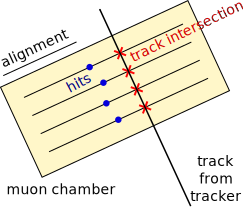
\includegraphics[width=\linewidth]{hip_explanation.pdf}

\column{0.7\linewidth}
\begin{enumerate}
\item align the tracker (Alessio's talk, yesterday)
\item propagate tracks from tracker to \mbox{muon layers\hspace{-1 cm}}
\item calculate unbiased residuals
\item adjust muon chambers to minimize \mbox{residuals\hspace{-1 cm}}
\end{enumerate}
\vspace{0.3 cm}
\end{columns}

\vspace{0.1 cm}
\item Tracker measurements dominate precision of most tracks anyway \\ (tracks with $p_T \lesssim 200$~GeV)
\item Decouples ``chicken-and-egg'' problem of alignment: track-fitting is independent of geometry updates \mbox{(no need for global fit or iteration)\hspace{-1 cm}}
\end{itemize}
\end{frame}

\begin{frame}
\frametitle{Sources of systematic error}

\begin{itemize}\setlength{\itemsep}{0.5 cm}
\item \textcolor{darkblue}{Tracker misalignments:} resolution, weak modes
\begin{itemize}\setlength{\itemsep}{0.1 cm}
\item use non-projective cosmic rays to look for distortions in tracker

\vspace{0.3 cm}
\begin{minipage}{1.2\linewidth}
\hspace{-2 cm}
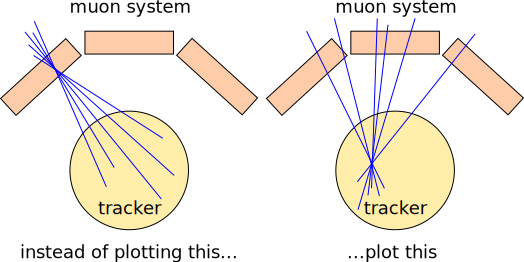
\includegraphics[height=3 cm]{tracker_xray.pdf}
\includegraphics[height=3 cm]{zresid_from_tracker_outerbottom.png}
\includegraphics[height=3 cm]{phiresid_from_tracker_inner_twist2.png}
\end{minipage}

\vspace{0.3 cm}
\item left: observation of TEC $z$ misalignment {\scriptsize (CRAFT\_V4, not latest)}
\item right: sensitivity study, tracker twist added by hand \textcolor{blue}{(blue)}
\end{itemize}

\item \textcolor{darkblue}{Propagation errors:} wrong $\vec{B}$-field, $dE/dx$, and track scattering
\begin{itemize}\setlength{\itemsep}{0.1 cm}
\item $\vec{B}$-field and $dE/dx$ errors have distinct dependences on charge and momentum (next slides)
\item scattering yields non-Gaussian outliers, accomodate with fit
\end{itemize}
\end{itemize}
\end{frame}



\begin{frame}
\frametitle{$\vec{B}$-field and misalignment}

\begin{columns}
\column{0.7\linewidth}
\vspace{-0.5 cm}
\begin{itemize}
\item Residuals from misalignment are independent of the tracks used to measure it
\item Residuals from $\vec{B}$-field errors flip sign with the charge
  of the muon and depend on $p_T$
\end{itemize}

\column{0.3\linewidth}
\vspace{0.5 cm}
\includegraphics[width=\linewidth]{antisymmetric_bfield.pdf}
\end{columns}

\vspace{-0.2 cm}
\textcolor{darkblue}{\large Two-bin approach:}
\begin{description}
\item[Fact:] momentum spectra for $+$ and $-$ charges are proportional
\item[Fact:] wrong $\vec{B}$-field and $dE/dx$ effects are antisymmetric with $q$
\end{description}

\begin{columns}
\column{0.5\linewidth}
\includegraphics[width=0.5\linewidth]{demo_momentum.pdf}
\includegraphics[width=0.5\linewidth]{demo_residual.pdf}

\column{0.6\linewidth}
\begin{itemize}
\item Find peak of residuals in two charge bins: $R_+$ and $R_-$
\item Average $(R_+ + R_-)/2$ is sensitive to misalignment only
\item Difference is sensitive to $\vec{B}$ error and $dE/dx$ errors
  only
\end{itemize}
\vspace{0.3 cm}
\end{columns}
\end{frame}

\begin{frame}
\frametitle{Demonstration in station 4}

\begin{itemize}
\item Station 4 has the largest $\vec{B}$-field errors: plot residuals across barrel
\item The \textcolor{darkred}{misalignment} breaks cleanly at the \mbox{chamber boundaries\hspace{-1 cm}}
\item The \textcolor{lightblue}{$\vec{B}$-field error} is independent of chamber
\end{itemize}

\includegraphics[height=\linewidth, angle=90]{demo_of_bfield.pdf}

\scriptsize grey background is the raw 2-D residuals distribution

linear fits are only a guide for the eye: not used in alignment!
\end{frame}

\begin{frame}
\frametitle{Residuals with new $\vec{B}(\vec{x})$ maps}
\begin{itemize}
\item Two new field maps available:
\begin{itemize}
\item scaling corrections from segments (data-based measurement)
\item new TOSCA simulation (consistent field lines)
\end{itemize}
\item Opportunity to test \textcolor{blue}{correctness of new $\vec{B}(\vec{x})$} and \textcolor{red}{insensitivity of alignment measure} with tracks propagated through new field
\begin{itemize}
\item left: histogram of bins from the previous plot (for all sectors)
\item right: how each bin changes when new field is applied
\end{itemize}
\end{itemize}

\vspace{-0.3 cm}
\mbox{ } \hfill {\tiny statistical errors in bins are ${\mathcal O}(\mbox{0.5~mm})$}

\only<1>{\includegraphics[width=4 cm, angle=90]{scaling_corrections_station4.pdf} \includegraphics[height=4 cm]{scaling_binbybin_station4.pdf}}
\only<2>{\includegraphics[width=4 cm, angle=90]{newgrid_corrections_station4.pdf} \includegraphics[height=4 cm]{newgrid_binbybin_station4.pdf}}
\end{frame}

\begin{frame}
\frametitle{Single-scattering}

\vspace{0.2 cm}
\begin{columns}
\column{0.65\linewidth}

\begin{itemize}
\item Non-multiple scattering processes have power-law distributions, while experimental resolution is Gaussian

\item Peak of residuals distribution should not be computed from
  the mean: it would be pulled by scattered ``outliers''

\item Model process as Lorentzian-Gaussian convolution:
\end{itemize}
\column{0.35\linewidth}
\includegraphics[width=\linewidth]{fitfunction.pdf}
\end{columns}

\vspace{0.45 cm}
\[ f(x) = \int_{-\infty}^\infty \frac{1}{\pi}\frac{\Gamma/2}{(x - \xi - \textcolor{darkblue}{x_0})^2 + (\Gamma/2)^2} \times 
\frac{1}{\sqrt{2\pi} \sigma} \exp\left(\frac{-\xi^2}{2 \sigma^2}\right) \, d\xi \]

\vspace{0.15 cm}
\hspace{-0.45 cm}
\begin{minipage}{\linewidth}
\begin{itemize}
\item Determine peak (alignment correction) from $\textcolor{darkblue}{x_0}$ of unbinned fit
\begin{itemize}\setlength{\itemsep}{0.1 cm}
\item regular mean ($\sum x_i/N$) = center of an unbinned Gaussian fit
\item this is the same thing, but with tails
\item ``outliers'' contribute far less to $f(x)$ log-likelihood \mbox{than Gaussian\hspace{-1 cm}}
\end{itemize}
\end{itemize}
\end{minipage}
\end{frame}

\begin{frame}
\frametitle{Is it a real alignment?}
\label{page:rphivsphi}

\hspace{-0.3 cm}
\begin{minipage}{\linewidth}
\begin{columns}
\column{0.5\linewidth}
\begin{itemize}
\item We want to find the real positions of chambers, not just minimize residuals
\item To look for biases in the track source, plot residuals \mbox{more finely\hspace{-0.5 cm}} than the chamber boundaries
\begin{itemize}
\item bias can change residuals shape inside chambers and across boundaries
\item only misalignments can make discontinuities at chamber boundaries
\end{itemize}
\item Cause of linear slopes in \mbox{$r\phi$ vs.\ $\phi$\hspace{-0.5 cm}} (bottom) under investigation {\scriptsize (DTs stretched in $x$?  tested $\phi_y$ and $z$-shift hypotheses\ldots)}

\item \mbox{Complete set of plots: \textcolor{blue}{\tt \tiny \href{http://indico.cern.ch/conferenceDisplay.py?confId=51267}{http://indico.cern.ch/conferenceDisplay.py?confId=51267}} \tiny (``more information'')\hspace{-10 cm}}
\end{itemize}

\column{0.6\linewidth}

\includegraphics[height=1.1\linewidth, angle=90]{alignmentplots_example1.pdf}

\includegraphics[height=1.1\linewidth, angle=90]{alignmentplots_example2.pdf}

\vspace{0.3 cm}
\end{columns}
\end{minipage}
\end{frame}

\begin{frame}
\frametitle{Cross-check: relative positions}

\begin{itemize}\setlength{\itemsep}{0.1 cm}
\item Alignment procedure determines chamber positions \mbox{relative to tracker\hspace{-1 cm}}
\item Chamber positions relative to other chambers is a true cross-check
\item Difference of residuals on the same track uses the track as a
  curved ruler to compare two chambers:

\mbox{ } \hfill \mbox{$\mbox{difference} = \big(\mbox{st.\ 3 track} - \mbox{st.\ 3 hit}\big) - \big(\mbox{st.\ 2 track} - \mbox{st.\ 2 hit}\big)$} \hfill \mbox{ }
\end{itemize}

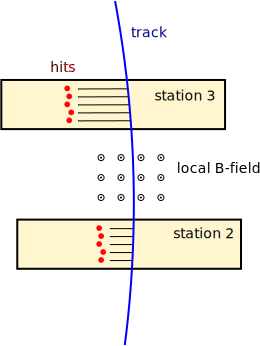
\includegraphics[height=4.4 cm]{residuals_difference.pdf} \includegraphics[width=4.5 cm, angle=90]{alignmentplots_example4.pdf}

\begin{itemize}
\item Difference distributions are about 4 times narrower than residuals
\end{itemize}
\end{frame}

\begin{frame}
\frametitle{Alignment results}

\begin{itemize}
\item The following are alignment corrections used in \mbox{CRAFT re-processing\hspace{-1 cm}}
\begin{itemize}
\item local $x$ is in the $r\phi$ direction, local $y$ is along the beamline
\item $x$ re-expressed as $\phi$ to demonstrate \mbox{lack of wheel rotations\hspace{-1 cm}}
\end{itemize}
\end{itemize}

\includegraphics[width=0.25\linewidth]{report2_xbywheel.png} \includegraphics[width=0.25\linewidth]{report2_phibywheel.png} \includegraphics[width=0.25\linewidth]{report2_y.png} \includegraphics[width=0.25\linewidth]{report2_phiz.png}

\begin{center}
\begin{tabular}{c c}
\textcolor{red}{aligned} in local $x$ and $\phi_z$: & \textcolor{red}{aligned} in local $y$: \\
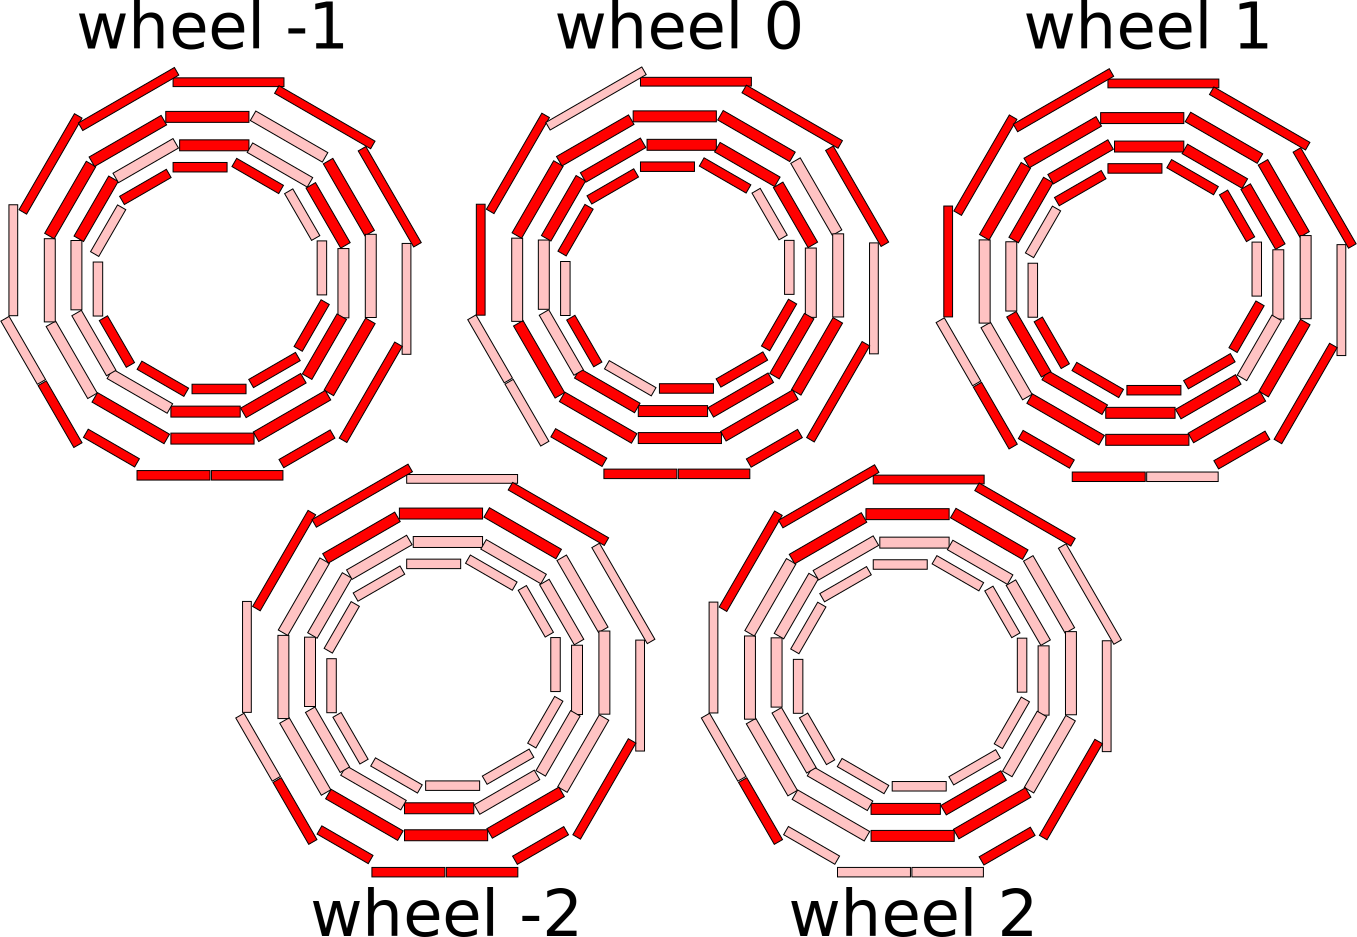
\includegraphics[width=0.4\linewidth]{aligned_rphi.pdf} & 
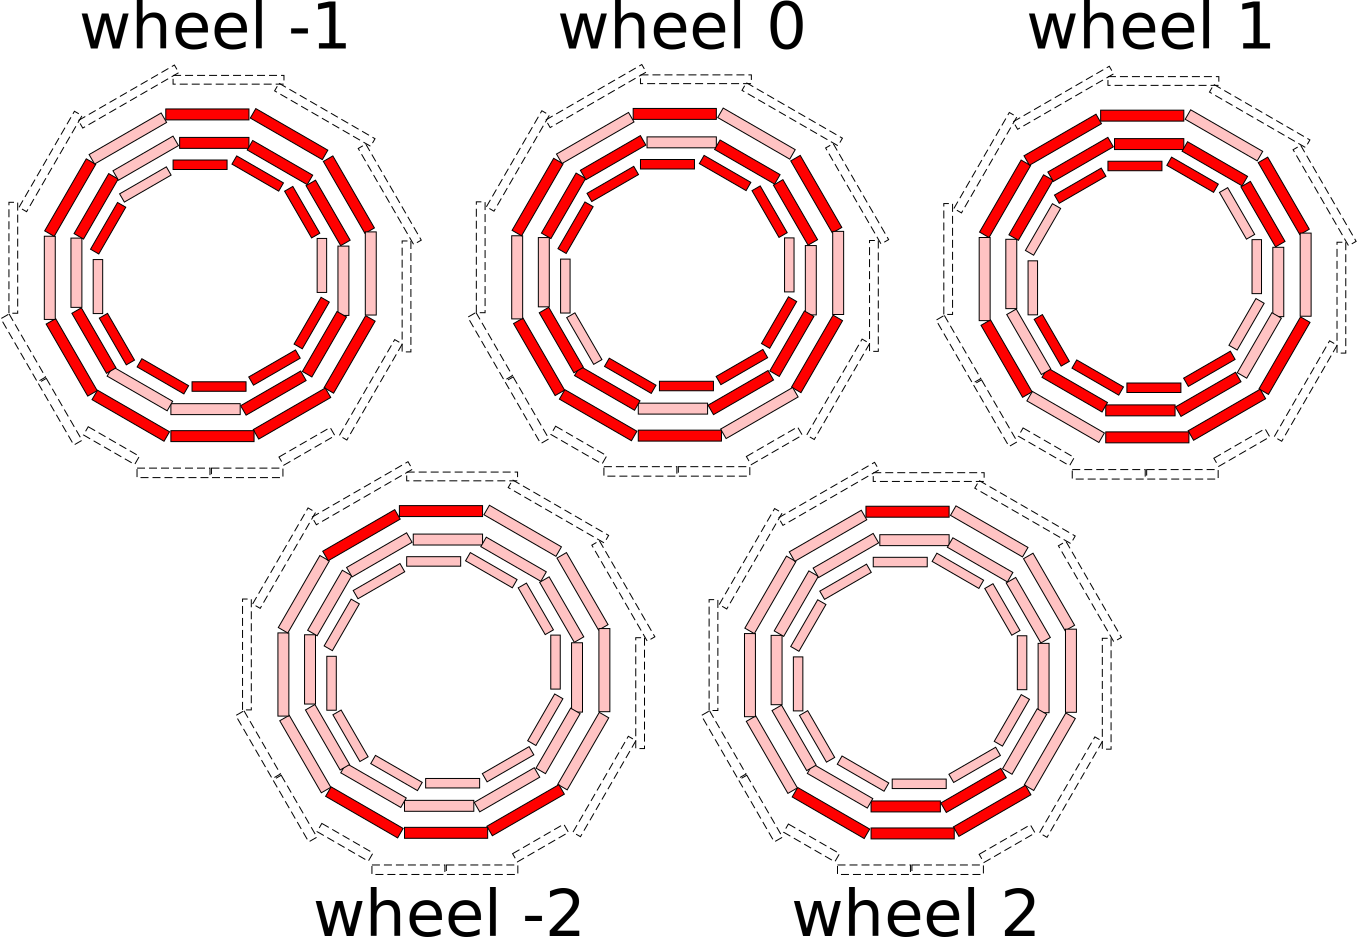
\includegraphics[width=0.4\linewidth]{aligned_z.pdf}
\end{tabular}
\end{center}
\end{frame}

\begin{frame}
\frametitle{Residuals after global alignment}

\begin{itemize}
\item Alignment narrowed and centered residuals distributions, as it must
\end{itemize}

\vspace{-0.2 cm}
\includegraphics[width=0.25\linewidth]{residuals_improvement1_relabled.pdf} \includegraphics[width=0.25\linewidth]{residuals_improvement2_relabled.pdf} \includegraphics[width=0.25\linewidth]{residuals_improvement3_relabled.pdf} \includegraphics[width=0.25\linewidth]{residuals_improvement4_relabled.pdf}

\begin{itemize}
\item Alignment preserved but didn't improve \mbox{residuals differences\hspace{-1 cm}}
\begin{itemize}
\item 1--2~mm {\it relative} chamber positions before and after alignment
\end{itemize}
\end{itemize}

\vspace{-0.2 cm}
\mbox{ } \hfill \includegraphics[width=0.25\linewidth]{residdiff12.pdf} \hfill \includegraphics[width=0.25\linewidth]{residdiff23.pdf} \hfill \includegraphics[width=0.25\linewidth]{residdiff34.pdf} \hfill \begin{minipage}{1 cm} \vspace{-1.3 cm} \tiny Note smaller scale \end{minipage} \mbox{ }

\vspace{0.3 cm}
\end{frame}

\begin{frame}
\frametitle{Cosmics track-splitting study}

\vspace{-0.05 cm}
\begin{columns}
\column{0.5\linewidth}
\begin{itemize}
\item Top and bottom half of a cosmic muon should have the same track parameters
\item GlobalMuon resolution worse than tracker-only for three reasons:
\begin{enumerate}
\item global misalignment
\item magnetic field errors
\item tracker given too little weight in global track fit
\end{enumerate}
\item Alignment improves matching of \mbox{$p_T > 100$~GeV cosmics\hspace{-1 cm}}
\begin{itemize}
\item insensitive to \textcolor{darkblue}{(2)}
\item plotted before \textcolor{darkblue}{(3)} \mbox{corrected\hspace{-1 cm}}
\end{itemize}
\item This is another cross-check because top-bottom agreement not used in \mbox{alignment procedure\hspace{-1 cm}}
\end{itemize}
\vspace{0.5 cm}

\column{0.6\linewidth}
\mbox{ } \hfill \textcolor{darkblue}{\scriptsize N.~Tran, A.~Bonato} \hfill \hfill \mbox{ }

\includegraphics[width=\linewidth]{plots_dphi.png}

\includegraphics[width=\linewidth]{plots_dpt.png}
\end{columns}
\end{frame}

\begin{frame}
\frametitle{Next steps in alignment}

\begin{enumerate}
\item Incorporate what we've learned into well-organized \mbox{alignment package\hspace{-1 cm}}
\begin{itemize}
\item \mbox{\scriptsize \tt Alignment/MuonAlignmentAlgorithms MuonAlignmentFromReference\hspace{-5 cm}}

{\scriptsize (CVS tag used for CRAFT alignment: V00-03-01)}

\item \mbox{\scriptsize \tt Alignment/CommonAlignmentMonitor AlignmentMonitorMuonSystemMap\hspace{-5 cm}}
\end{itemize}
\item Solve ``$r\phi$ residual vs.\ $\phi$'' problem (page~\pageref{page:rphivsphi}), if possible
\addtocounter{enumi}{-1}
\item Re-align accessible chambers of barrel in all 6 degrees of freedom
\item Use standAloneMuons to align those DT chambers which are inaccessible to globalMuons
\item Use standAloneMuons to align CSCs, using barrel as reference
\item Do it all again in CRAFT-2009, but as a push-button procedure
\end{enumerate}

\begin{center}
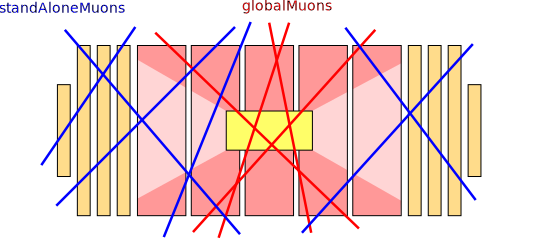
\includegraphics[width=0.65\linewidth]{accessible_to_globalMuons.pdf}
\end{center}
\end{frame}

\begin{frame}
\frametitle{Merging alignment information}

\begin{columns}
\column{0.45\linewidth}
\includegraphics[width=\linewidth]{disk_bending.png}

\column{0.63\linewidth}
\begin{itemize}
\item Straight-line monitors measure bending in endcap disks: $z$ and $\phi_x$ parameters
\begin{itemize}
\item included in CRAFT alignment
\item can measure $x$ and $\phi_z$ for some chambers
\end{itemize}
\item Track-based measurement of $x$, $\phi_y$, and $\phi_z$ will be more complete and precise
\begin{itemize}
\item can also measure $z$ and $\phi_x$
\end{itemize}
\item Combine results \mbox{parameter-by-parameter:\hspace{-1 cm}}
\begin{enumerate}
\item hardware prepares aligned CSCAlignmentRcd, passes it on
\item track-based doesn't update $z$, $\phi_x$
\end{enumerate}
\item Final result is easier to understand than a combined or constrained fit
\item Redundant measurements ($x$, $z$, $\phi_z$) reserved for cross-checks
\end{itemize}
\end{columns}
\end{frame}

\begin{frame}
\frametitle{Conclusions}

\begin{itemize}\setlength{\itemsep}{0.3 cm}
\item First global alignment, connecting muon chambers to the tracker's coordinate system
\item Careful to avoid errors due to source of tracks and propagation
\item Employed multiple cross-checks:
\begin{itemize}\setlength{\itemsep}{0.1 cm}
\item redundant binning shows no distortion inside of chambers
\item aligned in absolute coordinates, checked relative differences
\item track-splitting study showed improvement
\end{itemize}
\item Highly detailed misalignment scenario generated from this
  information, to be used in CRAFT Monte Carlo production
\item Wrapping this all up into a routine procedure
\begin{itemize}
\item to extend alignment into the endcap
\item and be ready for CRAFT-2009
\end{itemize}
\end{itemize}

\label{numpages}
\end{frame}






%% \begin{columns}
%% \column{0.63\linewidth}
%% 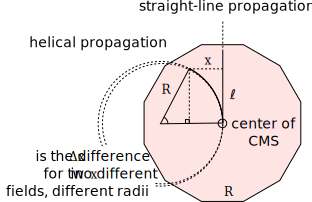
\includegraphics[width=\linewidth]{bfield_diagram.pdf}

%% \column{0.4\linewidth}
%% \mbox{Residuals from field error $\Delta B_z$:\hspace{-1 cm}}
%% \[ \Delta x = \frac{\ell^2 \, \, \Delta B_z}{2 \cdot \mbox{300 cm}} \, \left(\frac{q}{p_T}\right) \]

%% \begin{itemize}
%% \item misalignment residuals are \mbox{independent of tracks\hspace{-1 cm}}
%% \item $\vec{B}$-field residuals are linear in $(q/p_T)$
%% \end{itemize}
%% \end{columns}




%% \section*{First section}
%% \begin{frame}
%% \begin{center}
%% \Huge \textcolor{blue}{First section}
%% \end{center}
%% \end{frame}

\end{document}
